%----------------------------------------------------------------------------------------
%   PACKAGES AND OTHER DOCUMENT CONFIGURATIONS
%----------------------------------------------------------------------------------------

\documentclass[11pt,a4paper]{article}
\usepackage[utf8]{inputenc}
\usepackage[spanish]{babel}
\usepackage{amsmath}
\usepackage{amsfonts}
\usepackage{amssymb}
\usepackage{graphicx}
\usepackage{hyperref}
\usepackage{float}
\usepackage{multirow}
\usepackage{multicol} 
\usepackage[table,xcdraw]{xcolor}
\usepackage[colorinlistoftodos]{todonotes}
\author{Adrián Rodríguez Grillo - 100316457 \\
Álvaro Romero Díaz - 100316900}

% Margins
\topmargin=-0.45in
\evensidemargin=0in
\oddsidemargin=0in
\textwidth=6.5in
\textheight=9.0in
\headsep=0.25in

\begin{document}

\begin{titlepage}

\newcommand{\HRule}{\rule{\linewidth}{0.5mm}} % Defines a new command for the horizontal lines, change thickness here

\center % Center everything on the page
 
%----------------------------------------------------------------------------------------
%   HEADING SECTIONS
%----------------------------------------------------------------------------------------

\textsc{\LARGE Universidad Carlos III}\\[1.5cm] % Name of your university/college
\textsc{\Large Aprendizaje automático}\\[0.5cm] % Major heading such as course name
\textsc{\large Ingeniería informática}\\[0.5cm] % Minor heading such as course title

%----------------------------------------------------------------------------------------
%   TITLE SECTION
%----------------------------------------------------------------------------------------

\HRule \\[0.4cm]
{\huge \bfseries Práctica 3: Aprendizaje por refuerzo}\\[0.4cm] % Title of your document
\HRule \\[1.5cm]
 
%----------------------------------------------------------------------------------------
%   AUTHOR SECTION
%----------------------------------------------------------------------------------------

\begin{minipage}{0.4\textwidth}
\begin{flushleft} \large
\emph{Autor:}\\
\textsc{Adrián Rodríguez Grillo - 100316457} % Your name
\end{flushleft}
\end{minipage}
~
\begin{minipage}{0.3\textwidth}
\begin{flushright} \large
\emph{Autor:}\\
\textsc{Álvaro Romero Díaz - 100316900}
\end{flushright}
\end{minipage}\\[2cm]

%----------------------------------------------------------------------------------------
%   DATE SECTION
%----------------------------------------------------------------------------------------

{\large \today}\\[2cm] % Date, change the \today to a set date if you want to be precise

%----------------------------------------------------------------------------------------
%   LOGO SECTION
%----------------------------------------------------------------------------------------


\includegraphics[scale=1]{images/logo.jpg} \\[1cm] % Include a department/university logo - this will require the graphicx package
 
%----------------------------------------------------------------------------------------

\vfill % Fill the rest of the page with whitespace

\end{titlepage}

\tableofcontents
\newpage

\section{Introducción}
Este documento recoge la memoria de la práctica final de Aprendizaje Automático y qué está basada en aprendizaje por refuerzo.
En este documento pretendemos reflejar todos los pasos realizados para conseguir un agente que mediante una serie de pautas dadas por Q-learning, aprenda de manera automática cuál es el movimiento más conveniente en cada estado.

\paragraph{}
Por tanto, en este documento, lo primero que haremos será discutir las variables que recogeremos para el estudio de las instancias para, posteriormente, pasar a la explicación de clasificación de la mismas, en el proceso conocido como clusterización.

Tras esto, trataremos todo lo relacionado con el aprendizaje basado en instancias, explicando el funcionamiento de las funciones de pertenencia y similaritud, la primera que clasifica la situación actual dentro de un cluster y, la segunda, que la compara con las instancias del cluster para elegir la más similar y realizar su misma acción.

Finalmente, se descutirá sobre los resultados obtenidos, se responderá a las preguntas planteadas y se realizará una conclusión del trabajo.

\section{Definición de estados}

Realmente esta ha sido una de las partes que más problemas nos ha dado, ya que es bastante difícil encontrar atributos que den información real a Pac-man del mundo. Había que tener en cuenta los posibles valores de los atributos, dado que cuantos más valores posibles, más estados reales se podían crear.
Hay que destacar que hay estados poco probables o imposibles, más adelante veremos algunos ejemplos.

\subsection{Versión 1}

\begin{table}[H]
\centering
\label{atributosV1}
\begin{tabular}{|l|l|l|l|}
\hline
\multicolumn{4}{|c|}{\textbf{Atributos}}                           \\ \hline
NorteDisponible & SurDisponible & EsteDisponible & OesteDisponible \\ \hline
\end{tabular}
\caption{Atributos utilizados en la primera versión}
\end{table}

En esta primera versión quisimos representar los estados simplemente con las acciones disponibles, aplicando combinatoria básica sacamos que el número de estados posibles es 24. Tener un número pequeño de estados puede suponer ventaja pero no en este caso, ya que como apreciamos no recogemos información para favorecer al Q-learning dado que todos los atributos que recogemos trabajan sobre el presente, es decir, facilitan información al estado actual. En este caso solo aportan los movimientos posibles. 
Por lo mencionado en el párrafo anterior, descartamos dicha versión e hicimos una nueva.

\subsection{Versión 2}

\begin{table}[H]
\centering
\label{atributosV2}
\begin{tabular}{|l|l|l|l|l|}
\hline
\multicolumn{5}{|c|}{\textbf{Atributos}}                                                     \\ \hline
NorteDisponible & SurDisponible & EsteDisponible & OesteDisponible & DireccionFantasmaCerano \\ \hline
\end{tabular}
\caption{Atributos utilizados en la segunda versión}
\end{table}

Como se aprecia en la tabla, añadimos un nuevo atributo que representa hacia donde tiene que tirar nuestro Pac-man para avanzar hacia el fantasma más cercano. Por lo tanto, dicho atributo tiene cuatro posibles valores, lo cual hace que aumente el número de estados hasta 64 (24*4). 
Gracias a este atributo, Pac-man conoce un poco más el “futuro” y no solo le aportamos información del estado actual. A pesar de esto, decidimos seguir modificando los estados para seguir realizando pruebas.

\subsection{Versión 3}

\begin{table}[H]
\centering
\label{AtributosV3}
\begin{tabular}{|l|l|ll}
\hline
\multicolumn{4}{|c|}{\textbf{Atributos}} \\ \hline
NorteDisponible & SurDisponible & \multicolumn{1}{l|}{EsteDisponible} & \multicolumn{1}{l|}{OesteDisponible} \\ \hline
DireccionFantasmaCerano & DistanciaDiscretizada &  &  \\ \cline{1-2}
\end{tabular}
\caption{Atributos utilizados en la tercera versión}
\end{table}
En esta tercera versión, añadimos la distancia discretizada al fantasma más cercano. Esto a nuestro criterio podría aportar algo de valor, pasamos de tener 64 estados a tener 256. En el tratamiento de los datos explicaremos qué realizamos con dicho atributo.
Haciendo un análisis teórico fue cuando realmente nos dimos cuenta de que este atributo era irrelevante y solo iba a ser usado para calcular el refuerzo obtenido en cada paso (de esto se hablará más adelante).

\subsection{Versión 4}

\begin{table}[H]
\centering
\label{AtributosV4}
\begin{tabular}{|l|l|ll}
\hline
\multicolumn{4}{|c|}{\textbf{Atributos}} \\ \hline
NorteDisponible & SurDisponible & \multicolumn{1}{l|}{EsteDisponible} & \multicolumn{1}{l|}{OesteDisponible} \\ \hline
DireccionFantasmaCerano & FantasmasVivos &  &  \\ \cline{1-2}
\end{tabular}
\caption{Atributos utilizados en la cuarta versión}
\end{table}
Cuarta y penúltima versión, añadimos como atributo en cada estado el número de fantasmas vivos en ese instante. Con esto pensábamos que ganábamos información, pasamos de tener 56 estados (versión 2) a tener 256 de nuevo. 
Tras razonar, pensamos que estábamos mezclando de nuevo atributos necesarios para calcular el refuerzo y atributos necesarios para representar los estados, por lo tanto decidimos enviar un email al profesor de prácticas José Carlos González para que nos sacase de dudas. Su respuesta fue clara, no hacía falta meter dicho atributo en los estados y por lo tanto procedimos a borrarlo.

\subsection{Versión final}
La versión final, como ya se ha ido vaticinando, es la versión 2.

\begin{table}[H]
\centering
\label{AtributosVF}
\begin{tabular}{|l|l|l|l|l|}
\hline
\multicolumn{5}{|c|}{\textbf{Atributos}}                                                     \\ \hline
NorteDisponible & SurDisponible & EsteDisponible & OesteDisponible & DireccionFantasmaCerano \\ \hline
\end{tabular}
\caption{Atributos utilizados en la primera versión}
\end{table}

En esta versión recogemos los atributos que consideramos necesarios como mínimo para representar un estado. Toda la práctica desarrollada a partir de este punto parte de esta definición de estados.

\section{Tratamiento de los datos}

Para la versión 3 de la definición de estados tuvimos que discretizar los datos, es decir, que el atributo solo tuviese cuatro posibles valores. A pesar de que la distancia al fantasma cercano puede ir desde 0 hasta un número finito, discretizamos dicho atributo dando como posible valor un número natural comprendido entre 1 y 4 (ambos excluidos), donde el más cercano es el grupo 1 y el más lejano el grupo 4.

Mediante bucles if y unos rangos creados a nuestro criterio en Python realizamos dicha discretización, que a pesar de haber sido descartada como atributo, la usaremos en la función de refuerzo. Por tanto, los rangos han sido:

\begin{enumerate}
\item Distancia de 0 a 3 con el fantasma.
\item Distancia de 3 a 8 con el fantasma.
\item Distancia de 8 a 15 con el fantasma.
\item Distancia mayor de 15 con el fantasma.
\end{enumerate}

\section{Descripción del código}

Para la implementación del agente de aprendizaje basado en Q-Learning en el programa de python lo que hemos hecho ha sido crear un nuevo agente, llamado \textit{AgentQLearning}, que será el llamado desde el comando de iniciación del programa para su funcionamiento. Aunque es cierto que había ciertos métodos proporcionados en un principio decidimos desecharlos porque no podíamos reutilizar nada de lo proporcionado.

Por tanto, las clases utilizadas para la creación de nuestro agente han sido:

\begin{itemize}

\item\textbf{bustersAgents.py}: Que es donde se encuentra el controlador principal donde se llaman a los métodos auxiliares.

\item\textbf{extractData.py}: Que es el que obtiene los datos de la partida para ser usados posteriormente.

\item\textbf{saveData.py}: Que guarda en un .txt la información de la partida.

\item\textbf{tableOperators.py}: Que se encarga de realizar las operaciones sobre la tabla Q.

\item\textbf{refuerzo.py}: Que se encarga de calcular el refuerzo obtenido al ejecutar la acción.

\item\textbf{qFunction.py}: Que calcula el valor que se establecerá en la tabla Q para un estado y acción determinada.

\item\textbf{sacarFila.py}: Saca la fila de la tabla Q en la que se sitúa la información del estado actual.

\end{itemize}

Para la implementación de la tabla Q decidimos usar archivos JSON para guardar los datos del juego. Usaremos una matriz de dos dimensiones ($qtable(x,y)$) donde el primer [x] indicará el estado en el que se encuentra el Pac-Man.
La segunda [y] será una lista con los Q valores para las diferentes acciones disponibles de forma que las posiciones de la lista significarán:

\begin{itemize}
\item Posición 0 $\longrightarrow$ north
\item Posición 1 $\longrightarrow$ south
\item Posición 2 $\longrightarrow$ east
\item Posición 3 $\longrightarrow$ west
\end{itemize}


\subsection{tableOperators.py}

Esta clase será la que contiene todos lo métodos que actúan sobre la tabla Q del agente, siendo estas la creación, lectura y modificación. Estos métodos son una modificación de los creados en el tutorial 4 adaptados a los estados de esta práctica. Podemos encontrar los siguientes métodos:

\begin{itemize}

\item\textbf{Creator(filas)}: Crea la tabla Q vacía con tantas filas como se le introduzca por parámetro, este será el número de estados y la guarda en un fichero.

\item\textbf{readQtable()}: Lee la tabla Q y lo devuelve en forma de matriz.

\item\textbf{writeQtable(qtable)}: Recibe como parámetro la tabla Q en forma de matriz y la guarda en el archivo.

\item\textbf{computeQValueFromValues(state, action)}: Recibe el estado, fila en la matriz, y la acción realizada y devuelve el Q valor de dicha tupla.

\item\textbf{computeActionFromValues(state)}: Recibe como parámetro el estado en el que se encuentra el Pac-Man, es decir, el número de fila de la matriz que representa el estado, y devuelve la acción que aporta maximiza el Q valor.

\item\textbf{maxQValor(state)}: Recibe como parámetro el estado en el que se encuentra el Pac-Man, es decir, el número de fila de la matriz que representa el estado, y devuelve el Q valor más alto del estado. Es utilizado para la función que actualiza el Q valor.

\end{itemize}

\subsection{extractData.py}

Esta clase es la encarga de recoger los datos de la partida para que luego puedan ser utilizados para calcular el refuerzo de la acción y la actualización de la tabla Q. Este recibirá como parámetros el estado de juego (\textit{Gamestate}) y la información del fantasma más cercano.

\paragraph{}

En este método sacamos los datos de la partida anteriormente explicados para definir el estado, es decir, los movimientos que están disponibles y la dirección del fantasma más cercano al Pac-Man. También recogemos el número de fantasma vivos en dicho turno, que utilizaremos para la función de refuerzo, la fila a la que corresponde el estado del turno y el movimiento realizado en el turno. Todos estos datos serán utilizados posteriormente.

\paragraph{}
Debido a que el refuerzo se calcula con los datos del estado del que partimos, el movimiento y el estado al que transitamos, recurrimos en esta clase a una técnica utilizada en las practicas anteriores para que los cálculos se realicen correctamente. Dejamos correr un turno para poder obtener los datos del turno anterior y del actual y, a partir de ahí, empezar el proceso de aprendizaje.

Una vez obtenidos los datos de los dos estados, la acción realizada y el número de fantasmas vivos en cada turno llamamos al método que calcula el refuerzo. Tras esto, eliminamos el estado más antiguo de los datos para evitar el crecimiento del array que guarda los estados y datos.

\paragraph{}

Finalmente, este método devuelve la fila de la matriz del estado del que transitamos, la fila del estado al que transitamos y el refuerzo obtenido por el movimiento.

En esta clase también contamos con un método que transforma la acción en el valor utilizado por la matriz de la tabla Q para poder sacar correctamente la acción.

\subsection{sacarFila.py}

Esta clase se encarga de sacar la fila en la tabla Q del estado correspondiente introducido por parámetros. Es decir, en esta clase se introduce por parámetros los movimientos disponibles y la dirección en la que se encuentra el fantasma más cercano y gracias a un conjunto de ifs este estado es clasificado y se devuelve la linea de la matriz que le corresponde.

\subsection{refuerzo.py}

El refuerzo en nuestro agente depende de diferentes acontecimientos en el juego, cuando se realiza un movimiento que no mejora el estado de la partida se dará un refuerzo negativo mínimo, esto es así para evitar las estancación en bucles del agente, cuando se produce un coche con la pared, el refuerzo es altamente negativo. 

Sin embargo y, como hemos indicado anteriormente, cuando se produce una mejoría en la cercanía con los fantasmas, la cual se ha discretizado antes, se produce un refuerzo positivo mínimo, además, si se come un fantasma el refuerzo será ampliamente positivo.

\paragraph{}

Por tanto, esta es la clase que calcula el refuerzo al introducir como parámetros los estados implicados, el movimiento y el número de fantasmas vivos. Este, siguiendo las indicaciones interiores y, mediante comparaciones, devuelve el refuerzo.

\subsection{saveData.py}

Este método solo es utilizado en la Fase 1 de la practica para recoger y guardar los datos la partida en un fichero \textit{.txt}.

\subsection{qFunction.py}

Para la actualización de la tabla Q existente es necesario unos cálculos que dependen del estado del que transitamos, la acción realiza, el refuerzo, el valor Q máximo del estado al que transitamos y, como se trata de un proceso no determinista, de $\gamma$ y $\alpha$. Para ello seguimos la siguiente fórmula:

\begin{center}
$Q(s,a) \; \leftarrow \; (1 - \alpha) \, Q(s,a) \; + \; \alpha \, [ refuerzo \, + \, \gamma \, max_{a'} \, Q(s',a')]$
\end{center}

Este método recibirá como parámetros todos los datos necesarios y realizará los cálculos, devolviendo el valor actualizado de Q para el estado y la acción realizada.

\subsection{bustersAgents.py}

En esta clase es donde reside toda la lógica del agente, es la que se encarga de leer los datos de la tabla Q y de la partida, gestionarlos realizando los cálculos necesarios y los guarda de nuevo en el fichero de la tabla Q.

Un problema que detectamos fue que el refuerzo negativo cuando el Pac-Man se chocaba con una pared no se guardaba debido a que este se cerraba dando el error antes. La solución fue comprobar si el siguiente movimiento que realizaría el agente era legal, guardando el refuerzo negativo, si esto no era así, antes de que el programa se cerrase.

\paragraph{}

Por tanto, lo que realiza este método es: primero lee la tabla Q existente y extrae los datos de la partida. Si es el primer turno, lo deja pasar estando parado para poder empezar a calcular a partir del siguiente.

Tras esto, si el siguiente movimiento que realizará el Pac-Man es ilegal, actualizará la tabla Q con el refuerzo negativo que supone el coche con la pared. Por otro lado, si el movimiento es legal actualiza la tabla Q con los datos del refuerzo obtenido con el movimiento realizado y el cambio de estado.

\section{Descripción de asignación de estado empleada}

En esta parte del documento vamos a ver el porqué de los atributos elegidos para nuestros estados.
Todos nuestros estados tienen que aportar información a Pac-Man sobre el conocimiento del mundo, es decir, conocer de manera verídica la situación actual en la que se encuentra. Para ello lo primero que pensamos que era totalmente necesario, era saber hacia dónde podía tirar Pac-Man, esto se traduce en conocer qué movimientos hay disponibles en cada estado. Gracias a esto conseguimos nuestros cuatro primeros atributos, cada uno con dos posibles valores (Disponible o no disponible), alcanzando un total de 24 = 16 estados posibles. 

\paragraph{}
Ahora nuestro Pac-man conoce los movimientos disponibles que tiene en cada momento , pero no tiene ningún conocimiento que le indique en cierta medida hacia dónde ir, es decir, algo que le sirva de guía para conseguir lograr su objetivo, que es comerse a todos los fantasmas. Por lo tanto, llegamos a la conclusión de que podíamos añadir un atributo que indicase hacia donde tiene que tirar Pac-Man para acercarse al fantasma más cercano. 
Dicho atributo puede tener cuatro posibles valores (Norte, Sur, Este y Oeste), así que sumando estas posibilidades a todos los atributos anteriores, obtenemos 24*4 = 24*22 = 26 = 64 estados.
Este es el número mínimo de estados que hemos conseguido definir para implementar correctamente Q-learning. Tener el mínimo número de estados supone ciertas ventajas y desventajas.

\subsection{Ventajas}

Tener menos estados supone trabajar con menos atributos y por lo tanto hay que realizar menos implementación en Python, es más básico y se pueden hacer pruebas fácilmente.

\subsection{Desventajas}

Claramente 64 estados se pueden quedar escasos para cualquier mapa medianamente grande de Pac-man, ya que en muchos casos se repetirán los estados. Esto conlleva la modificación de los Q-valores de un mismo estado varias veces en la misma partida en caso de que se repitan los estados, es decir, modifica valores que nosotros ya habíamos actualizado anteriormente en la misma partida.

\paragraph{}
En mapas en los que se repitan pocos estados nuestro agente va a aprender rápido y fácil pero va a tener problemas en ciertos mapas, como por ejemplo en este tipo de túnel. 

\begin{figure}[H]
\centering
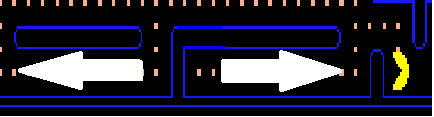
\includegraphics[scale=1]{images/estado.png}
\end{figure}


En este caso apreciamos que las flechas recogen el mismo estado:

\begin{table}[H]
\centering
\label{EstadoEjemplo}
\begin{tabular}{|c|c|}
\hline
\multicolumn{2}{|c|}{\textbf{Estado}} \\ \hline
NorteDisponible & NO \\ \hline
SurDisponible & NO \\ \hline
EsteDisponible & SI \\ \hline
OesteDisponible & SI \\ \hline
Fantasma+cercano & OESTE \\ \hline
\end{tabular}
\end{table}

Lo que está ocurriendo es que tenemos dos “túneles” donde Pac-man se encuentra en el mismo estado pero tiene que tomar caminos contrarios para alcanzar al fantasma. Esto es una gran desventaja ya que con la definición de nuestros estados y Q-learning resulta imposible que en una misma partida pudiese pasar por los dos “túneles” realizando los movimientos correctos.

Con lo cual llegamos a la conclusión de que no hubiese estado de más añadir algún atributo que hubiese aportado información complementaria como por ejemplo el número de fantasmas vivos, con esto hubiese sabido nuestro agente qué hacer en función del número de fantasmas que se haya comido ya. 

\end{document}